\documentclass[tikz, margin=0.1pt]{standalone}
\usepackage{tikz} 
\usepackage{pgfplots} % Include pgfplots package for plotting functions
\pgfplotsset{compat=1.17} % Set compatibility level

\begin{document}

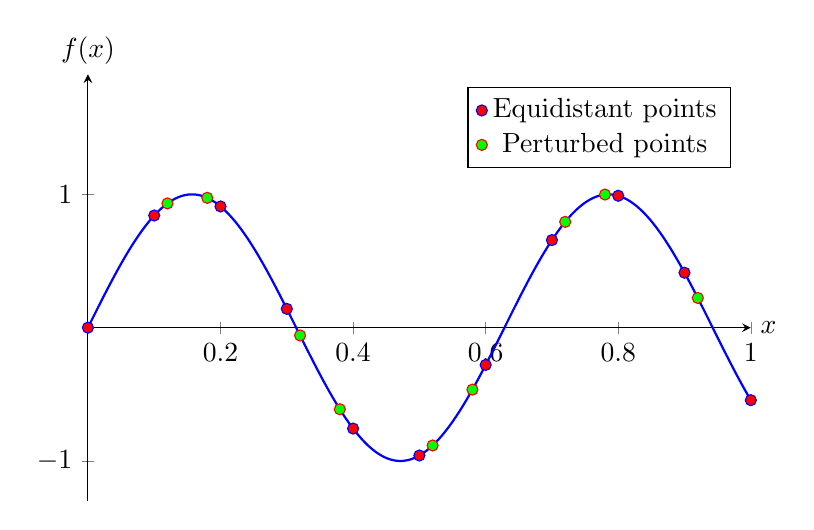
\begin{tikzpicture}[scale=1, dot/.style = {circle, fill, minimum size=#1, inner sep=0pt, outer sep=0pt}, dot/.default = 1pt] 
\begin{axis}[
    domain=0:1, % Domain of the function
    samples=100, % Number of samples for smooth curve
    axis lines=middle,
    xlabel=\(x\),
    ylabel=\(f(x)\),
    ymin=-1.3, ymax=1.9,
    xmin=0, xmax=1,
    every axis x label/.style={at={(ticklabel* cs:1)}, anchor=west},
    every axis y label/.style={at={(ticklabel* cs:1)}, anchor=south},
    width=10cm, height=7cm,
    legend pos=north east,
]

% Plot of the function f(x) = sin(10x)
\addplot[smooth, thick, blue, forget plot] {sin(deg(10*x))};

% Show equidistant points on the curve, i.e. the parameterization
\addplot+[only marks, mark=*, mark options={fill=red}] coordinates {
    (0.0, {sin(deg(10*0.0))})
    (0.1, {sin(deg(10*0.1))})
    (0.2, {sin(deg(10*0.2))})
    (0.3, {sin(deg(10*0.3))})
    (0.4, {sin(deg(10*0.4))})
    (0.5, {sin(deg(10*0.5))})
    (0.6, {sin(deg(10*0.6))})
    (0.7, {sin(deg(10*0.7))})
    (0.8, {sin(deg(10*0.8))})
    (0.9, {sin(deg(10*0.9))})
    (1.0, {sin(deg(10*1.0))})
};

\addlegendentry{Equidistant points}

% Add perturbed points on the curve, should not include the ends 
\addplot+[only marks, mark=*, mark options={fill=green}] coordinates {
    (0.1 + 0.02, {sin(deg(10*(0.1 + 0.02)))})
    (0.2 - 0.02, {sin(deg(10*(0.2 - 0.02)))})
    (0.3 + 0.02, {sin(deg(10*(0.3 + 0.02)))})
    (0.4 - 0.02, {sin(deg(10*(0.4 - 0.02)))})
    (0.5 + 0.02, {sin(deg(10*(0.5 + 0.02)))})
    (0.6 - 0.02, {sin(deg(10*(0.6 - 0.02)))})
    (0.7 + 0.02, {sin(deg(10*(0.7 + 0.02)))})
    (0.8 - 0.02, {sin(deg(10*(0.8 - 0.02)))})
    (0.9 + 0.02, {sin(deg(10*(0.9 + 0.02)))})
};

\addlegendentry{Perturbed points}

\end{axis}

\end{tikzpicture}

\end{document}
